\documentclass[border=10pt]{standalone}

\usepackage{tikz}
\usepackage{tikzsymbols}
\usetikzlibrary{calc,patterns,shapes.geometric}

\def\centerarc[#1](#2)(#3:#4:#5){\draw[#1] ($(#2)+({#5*cos(#3)},{#5*sin(#3)})$) arc (#3:#4:#5);}

\begin{document}
	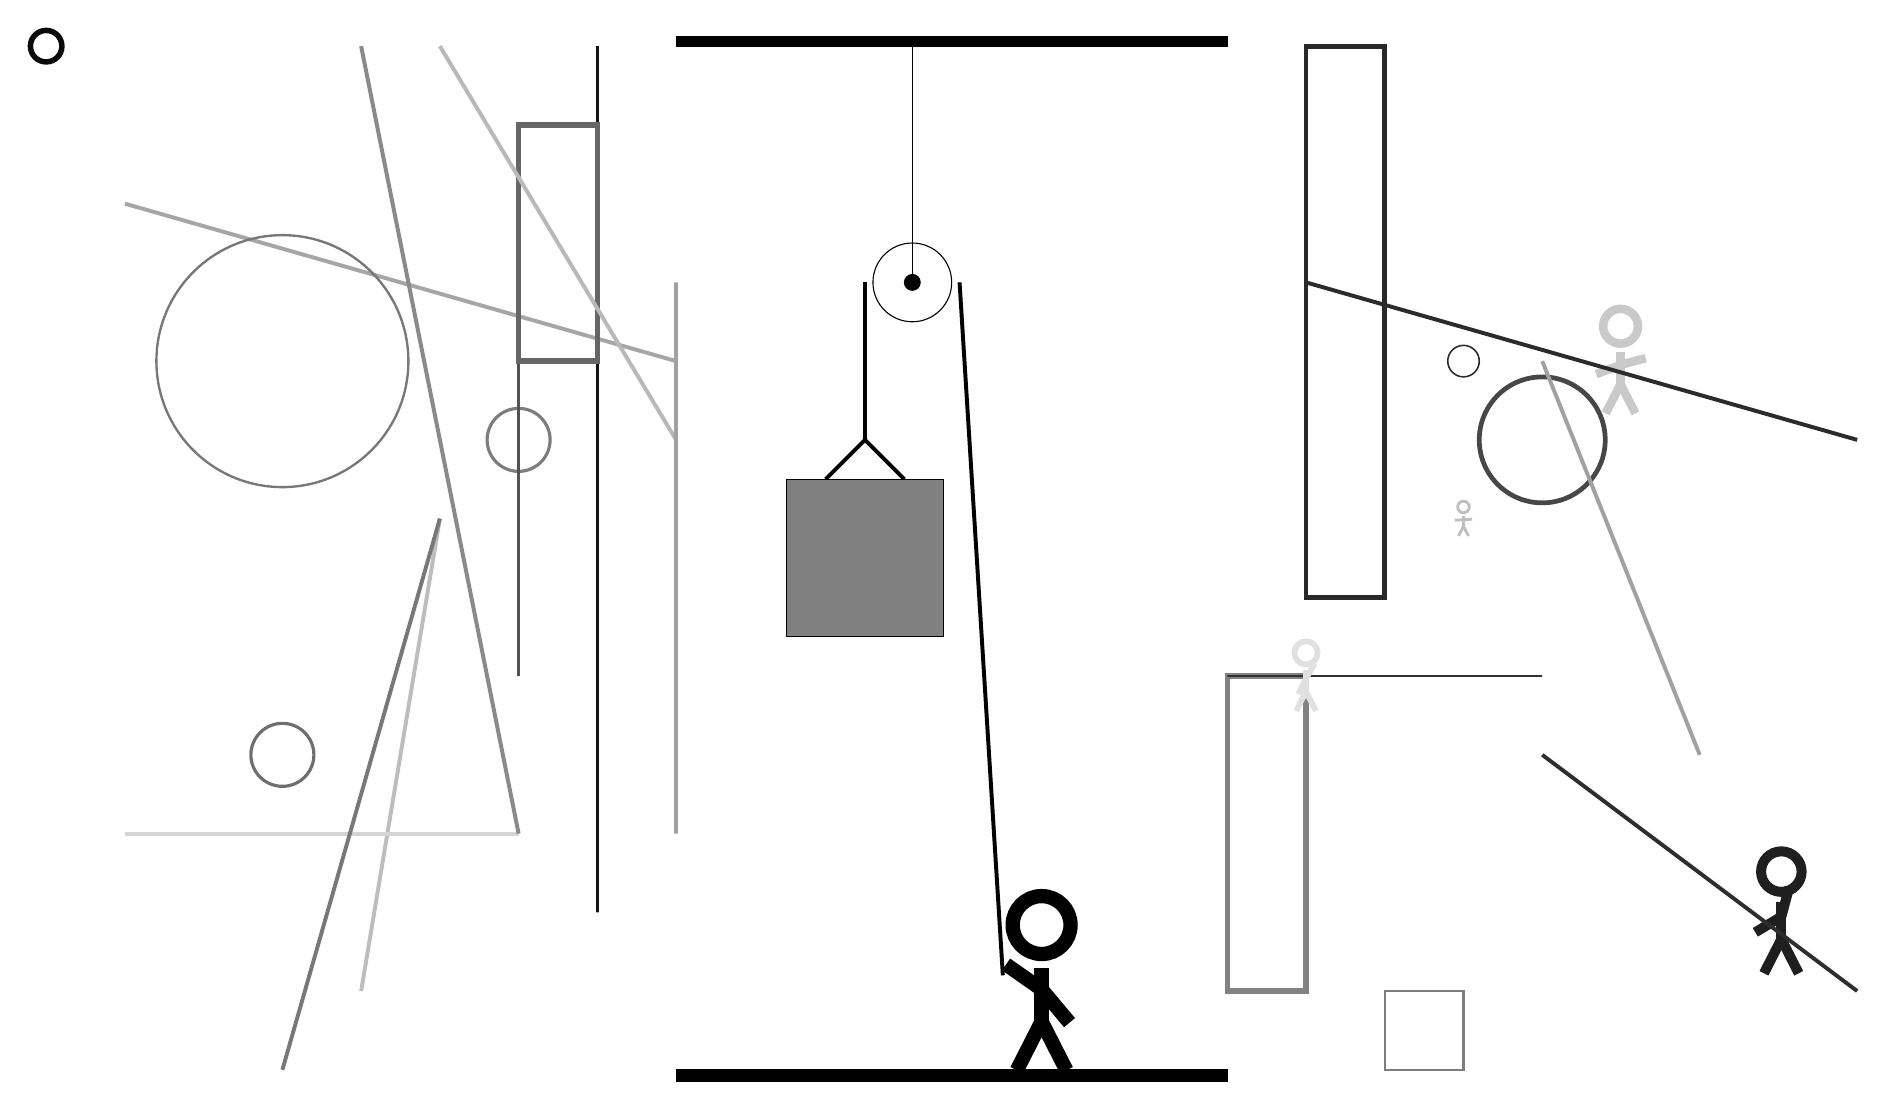
\begin{tikzpicture}
		%%%%% START %%%%%
		
		\draw[fill=black] (-2, 10) rectangle (5, 10.125);
		
		\node[line width=0.3mm, color=black!21] at (10, 6) {\Strichmaxerl[6][21][15]};
		
		\draw [line width=0.4mm, color=black!57](-7, 1) circle (0.4);
		\draw[line width=0.4mm, color=black!92] (-3, -1) rectangle (-3, 10);
		\node[line width=0.6mm, color=black!88] at (12, -1) {\Strichmaxerl[7][31][75]};
		
		\draw[line width=0.5mm, color=black!35](-2, 6) -- (-9, 8);
		
		\draw [line width=0.6mm, color=black!72](9, 5) circle (0.8);
		
		\draw [line width=0.4mm, color=black!51](-4, 5) circle (0.4);
		
		\draw[line width=0.5mm, color=black!26](-6, -2) -- (-5, 4);
		\draw [line width=0.6mm, color=black!67](7, 2) circle (0.0);
		
		\node[line width=0.6mm, color=black!25] at (8, 4) {\Strichmaxerl[2][2][5]};
		\draw[line width=0.5mm, color=black!17](-4, 0) -- (-9, 0);
		\draw[line width=0.5mm, color=black!53](-7, -3) -- (-5, 4);
		\draw [line width=0.5mm, color=black!10](5, -1) circle (0.0);
		
		\draw [line width=0.7mm, color=black!96](-10, 10) circle (0.2);
		\draw[line width=0.6mm, color=black!84] (6, 3) rectangle (7, 10);
		\draw[line width=0.7mm, color=black!49] (5, 2) rectangle (6, -2);
		\draw[line width=0.3mm, color=black!51] (7, -3) rectangle (8, -2);
		
		\draw[line width=0.3mm, color=black!68] (-4, 7) rectangle (-4, 2);
		\draw[line width=0.7mm, color=black!60] (-4, 6) rectangle (-3, 9);
		\draw[line width=0.5mm, color=black!83](6, 7) -- (13, 5);
		\draw[line width=0.5mm, color=black!82](9, 1) -- (13, -2);
		
		\draw[line width=0.5mm, color=black!36](-2, -3) -- (-2, -3);
		\draw [line width=0.3mm, color=black!53](-7, 6) circle (1.6);
		\draw[line width=0.3mm, color=black!81] (5, 2) rectangle (9, 2);
		\draw[line width=0.5mm, color=black!28](-2, 5) -- (-5, 10);
		
		\draw[line width=0.6mm, color=black!37] (-2, 7) rectangle (-2, 0);
		\draw [line width=0.2mm, color=black!83](8, 6) circle (0.2);
		\node[line width=0.3mm, color=black!12] at (6, 2) {\Strichmaxerl[4][63][60]};
		
		\draw[line width=0.5mm, color=black!46](-6, 10) -- (-4, 0);
		\draw[line width=0.5mm, color=black!37](9, 6) -- (11, 1);
		
		\draw (1, 7) circle (0.5);
		\draw[fill=black] (1, 7) circle (0.1);
		\draw (1, 10) -- (1, 7);
		
		\draw[line width=0.5mm] (-0.1, 4.5) -- (0.4, 5.0) -- (0.9, 4.5);
		\draw[fill=black!50] (-0.6, 4.5) rectangle (1.4, 2.5);
		
		\draw[line width=0.5mm] (0.4, 7) -- (0.4, 5.0);
		\centerarc[line width=0.5mm](1, 7)(0:180:0.6);
		\draw[line width=0.5mm](1.6, 7) -- (2.15, -1.8);
		
		\node at (2.6, -1.9) {\Strichmaxerl[10][-35][-50]};
		
		\draw[fill=black] (-2, -3) rectangle (5, -3.15);
		
		%%%%% END %%%%%
	\end{tikzpicture}
\end{document}